\section{Queueing networks}

Queueing theory is the study of what occurs when there are numerous tasks, limited resources, resulting in lengthy queues and delays.
Queueing network modeling is a specific method for computer system modeling. 
It represents the computer system as a network comprising queues.
\begin{definition}[\textit{Queueing networks}]
    A network of queues consists of service centers, representing system resources, and customers, representing users or transactions.
\end{definition}

Queueing theory comes into play whenever queues emerge. 
In computer systems, queues are ubiquitous:
\begin{itemize}
    \item The CPU utilizes a time-sharing scheduler.
    \item Disk operations involve a queue of requests awaiting block reads or writes.
    \item Routers manage queues of packets awaiting routing.
    \item Databases feature lock queues, where transactions await record locks.
\end{itemize}
Queueing theory aids in performance prediction, particularly for capacity planning, and is rooted in stochastic modeling and analysis.
The success of queueing networks lies in their ability to abstract low-level system details, focusing instead on high-level performance characteristics.

\paragraph*{Single queue}
In a single queue scenario, customers from a certain population arrive at a service facility.
This facility, equipped with one or more servers, provides the required service to customers.
If a customer cannot access a server immediately, they join a queue or buffer until a server becomes available.
Upon completion of service, the customer departs, and the server selects the next customer from the buffer based on the service discipline or queuing policy.

\subsection{Queueing model}
Queuing models encompass various aspects, including:
\begin{itemize}
    \item \textit{Arrival of customers}: customer arrivals represent jobs entering the system, detailing their frequency, speed, and types. 
        The average arrival rate, denoted as $\lambda$, is of interest.
        \begin{figure}[H]
            \centering
            \begin{subfigure}{0.32\textwidth}
                \centering
                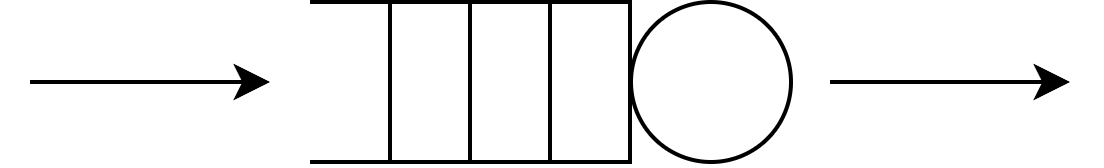
\includegraphics[width=1\linewidth]{images/ext.png} 
                \caption{Data from external source}
            \end{subfigure}
            \begin{subfigure}{0.32\textwidth}
                \centering
                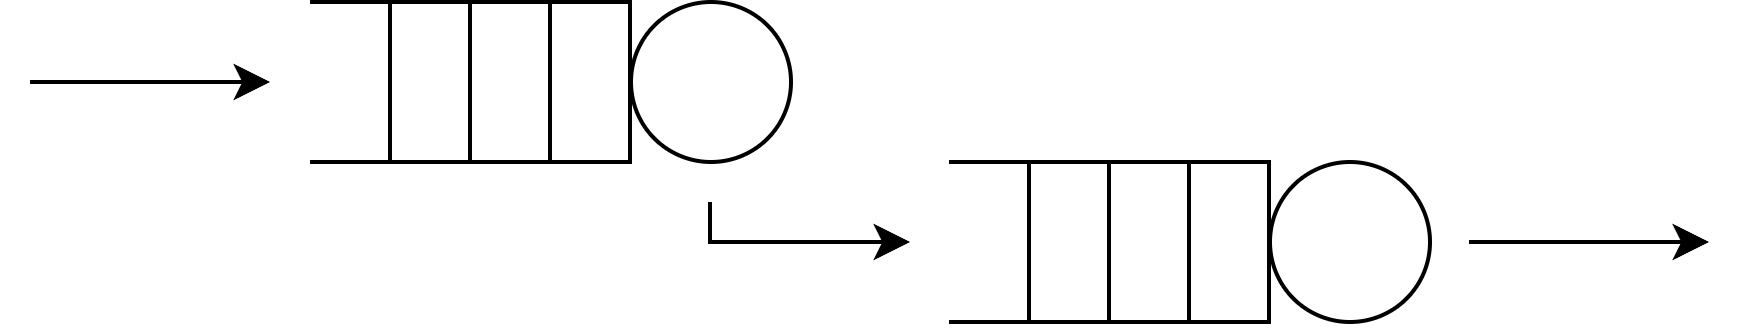
\includegraphics[width=1\linewidth]{images/ext1.png} 
                \caption{Data from another queue}
            \end{subfigure}
            \begin{subfigure}{0.32\textwidth}
                \centering
                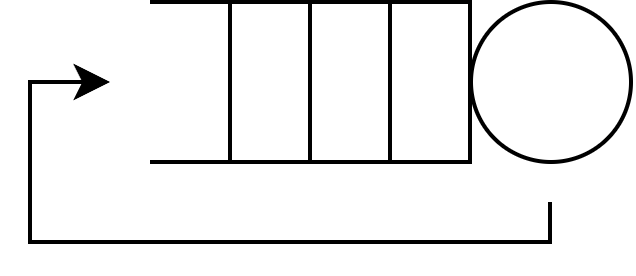
\includegraphics[width=0.6\linewidth]{images/ext2.png}
                \caption{Data from same queue}
            \end{subfigure}
            \caption{Types of data arrival}
        \end{figure}
    \item \textit{Service}: the service aspect represents the duration a job spends being served, indicating the time a server dedicates to satisfying a customer.
        Similar to inter-arrival time, the key characteristics of service time include its average duration and distribution function.
        If the average duration of a service interaction between a server and a customer is $\frac{1}{\mu}$, then $\mu$ represents the maximum service rate.
        Possible situations include:
        \begin{itemize}
            \item \textit{Single server}: the service facility can handle only one customer at a time. 
                Waiting customers remain in the buffer until selected for service, with the selection process depending on the service discipline.
            \item \textit{Infinite server}: there are always enough servers available for every arriving customer, eliminating queues and buffers.
            \item \textit{Multiple server facilities}: these facilities have a fixed number of servers, denoted as $c$, each capable of serving a customer simultaneously. 
                If the number of customers in the facility is less than or equal to $c$, there is no queueing, and each customer has direct access to a server. 
                However, if there are more than $c$ customers, the additional customers must wait in the buffer.
        \end{itemize}
    \item \textit{Queue}: if the number of jobs exceeds the system's parallel processing capacity, they queue in a buffer. 
        Customers unable to receive immediate service wait in the buffer until a server becomes available. 
        When the buffer reaches its finite capacity, two options arise:
        \begin{itemize}
            \item The facility being full is communicated to the arrival process, and arrivals are suspended until spare capacity is available, or a customer leaves.
            \item Arrivals continue, but incoming customers are turned away until spare capacity is available again.
        \end{itemize}
        If the buffer's capacity is so large that it never affects customer behavior, it's considered infinite. 
        When a job in service leaves the system, a job from the queue can enter the now vacant service center. 
        The service discipline or queuing policy dictates which job in the queue starts its service. 
        In cases where multiple customers are waiting, a rule determines which waiting customer gains access to a server next. 
        Common service disciplines include FCFS (First-Come-First-Serve or FIFO), LCFS (Last-Come-First-Serve or LIFO), RSS (Random-Selection-for-Service), and PRI (Priority), where different priorities are assigned to elements of a population.
    \item \textit{Population}: The characteristic of interest regarding the population is typically its size. 
        If the population size is fixed at a value $N$, no more than $N$ customers will ever require service simultaneously.
        When the population is finite, the arrival rate of customers is influenced by the number already in the service facility.
        If the population size is so large that it has no noticeable impact on the arrival process, we assume it to be infinite. 
        Ideally, members of the population are indistinguishable from one another.
        However, if they are not, we categorize the population into classes, where members exhibit similar behavior. 
        Different classes may differ in characteristics such as arrival rate or service demand. 
        Identifying these classes is part of workload characterization.
    \item \textit{Routing}: when a job completes service at a station and has multiple potential routes, a suitable selection policy must be established. 
        This policy, dictating how the next destination is chosen, is termed routing.
        Routing specifications are necessary at points where jobs leaving a station can have more than one destination.
        The main routing algorithms we will consider include:
        \begin{itemize}
            \item \textit{Probabilistic}: each path is assigned a probability of being chosen by the departing job.
            \item \textit{Round robin}: the destination selected by the job rotates among all possible exits.
            \item \textit{Join the shortest queue}: jobs can assess the queue length of potential destinations and opt for the one with the fewest waiting jobs to be served.
        \end{itemize}
\end{itemize}
For many systems, we can conceptualize the system as a collection of resources and devices, with customers or jobs circulating among them. 
Each resource in the system can be associated with a service center, and customers are routed among these service centers.
After receiving service at one service center, a customer may move on to other service centers based on a predefined pattern of behavior that corresponds to the customer's requirements.

\subsection{Classification}
A queueing network can be depicted as a graph, where nodes represent the service centers $k$ and arcs signify potential transitions of users from one service center to another.
Together, nodes and arcs define the network's topology.
\begin{figure}[H]
    \centering
    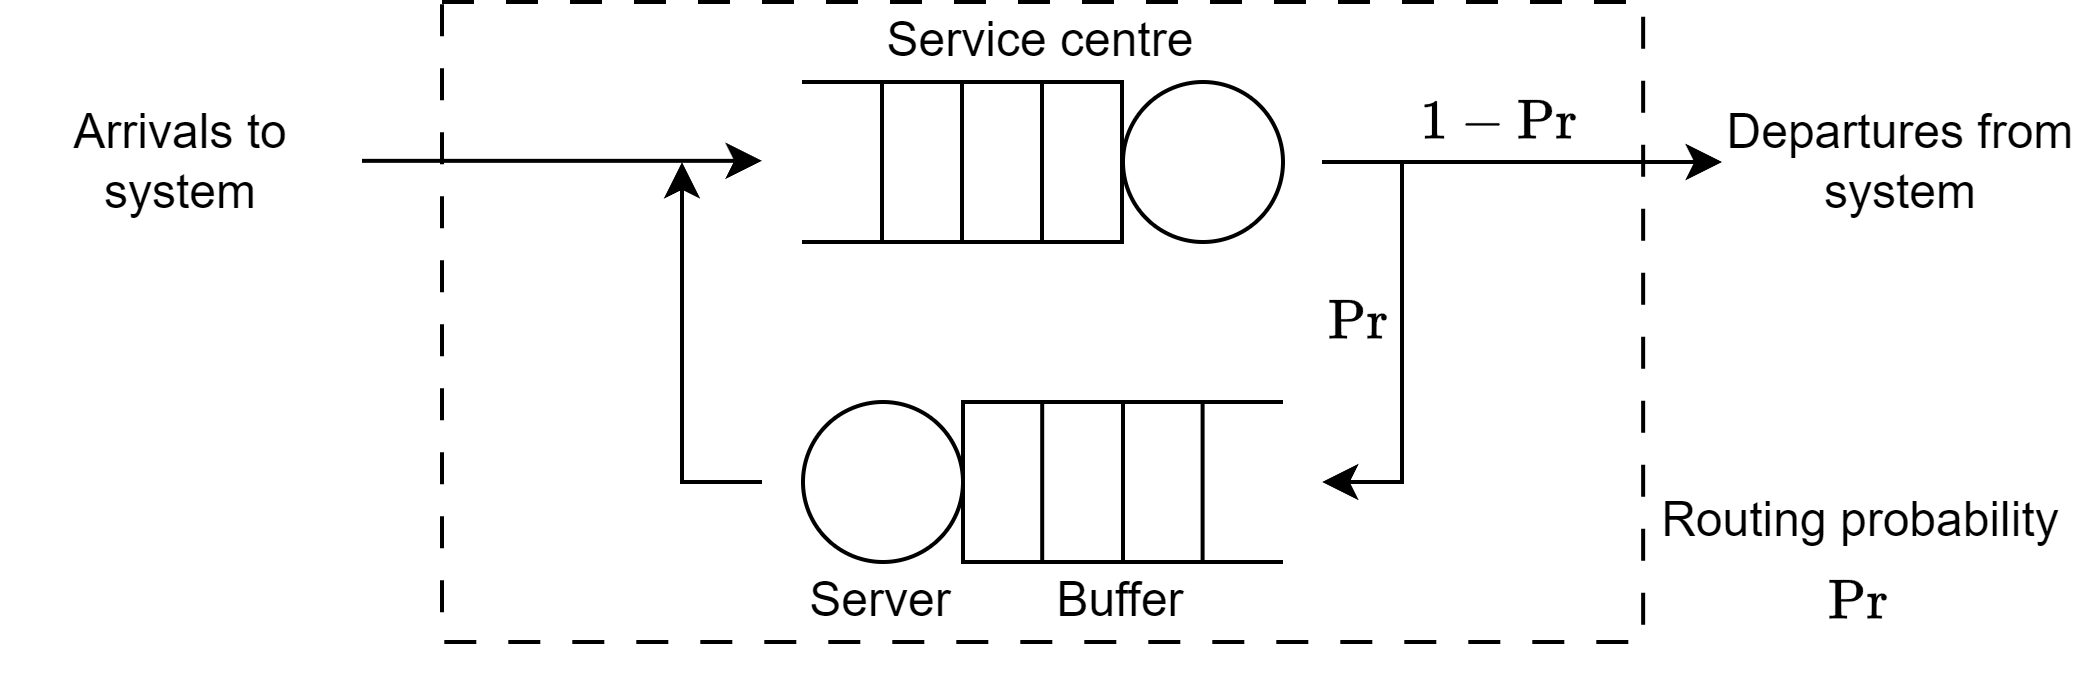
\includegraphics[width=0.65\linewidth]{images/per.png}
    \caption{Queueing network representation}
\end{figure}
A network may be:
\begin{itemize}
    \item \textit{Open}: customers may arrive from or depart to some external environment. 
        Open models are characterized by arrivals and departures from the system.
    \item \textit{Closed}: a fixed population of customers remains within the system. 
        In closed models, we have a parameter $N$ that accounts for the fixed population of jobs continuously circulating within the system.
    \item \textit{Mixed}: there are classes of customers within the system exhibiting open and closed patterns of behavior, respectively.
\end{itemize}

\paragraph*{Graphical notation}
Graphical notation is not standardized, but typically corresponds to a graph where edges represent the flow of customers in the network.
\begin{figure}[H]
    \centering
    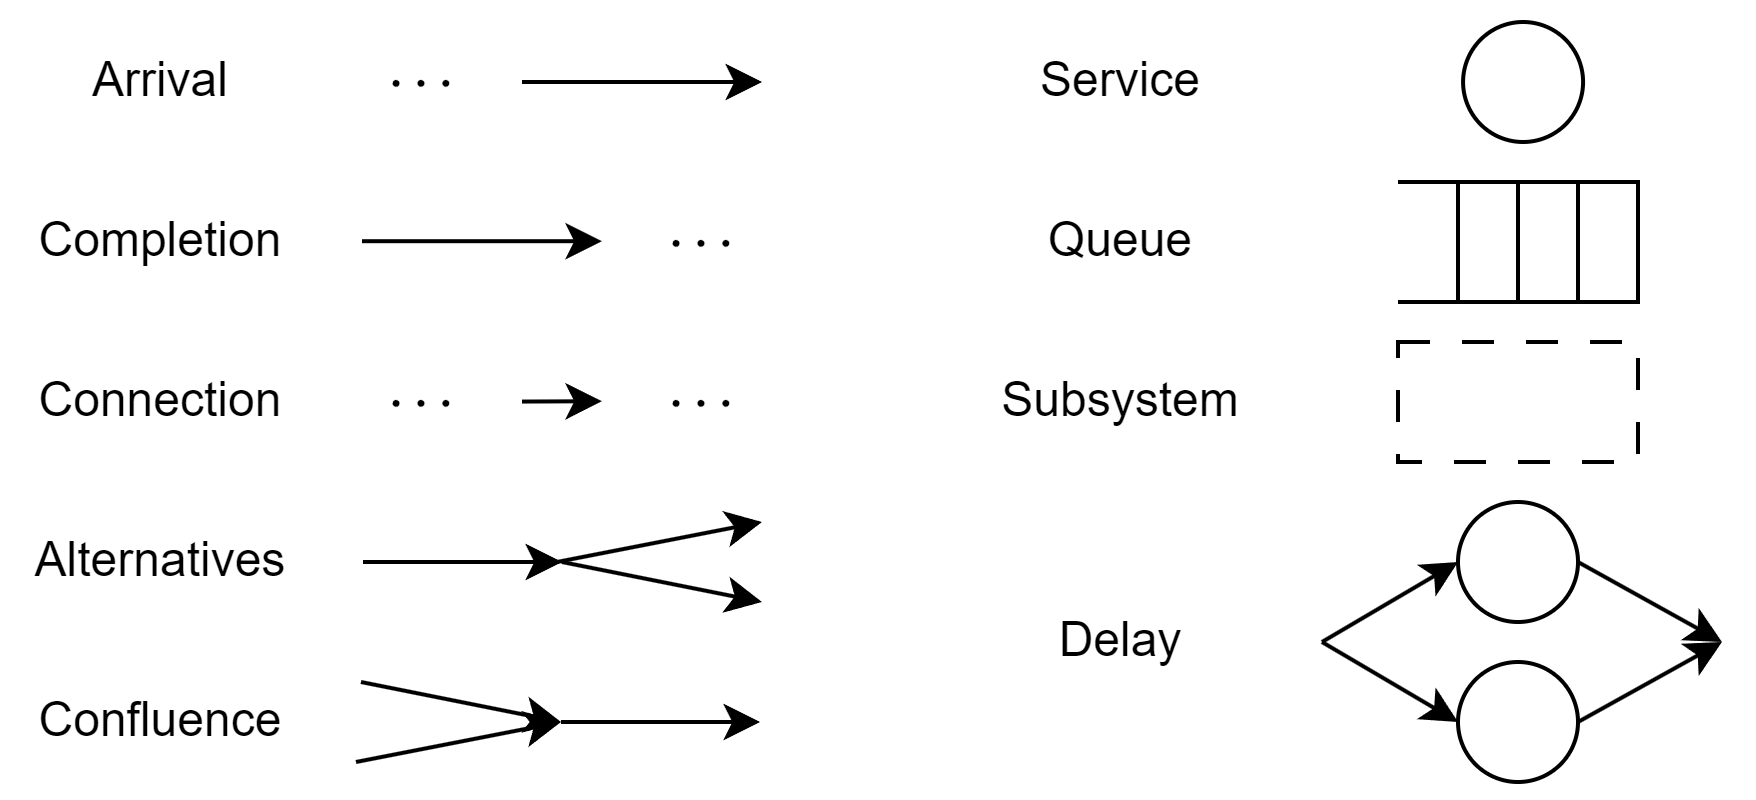
\includegraphics[width=0.5\linewidth]{images/gra.png}
    \caption{Graphical notation}
\end{figure}